\subsection{Notfall-Evakuierung mit einem Service-Roboter}
\label{subsec:evacuation}
    Mit dem Szenario der Notfall-Evakuierung wird ein weiterer Anwendungsfall definiert, welcher dabei helfen soll, die 
    Anforderungen zu identifizieren, die für die Bereitstellung des Frameworks der Steuerzentrale benötigt werden.
    \\
    \linebreak
    Objektiv betrachtet gibt es bei diesem Fall ebenso einen Auslöser, bspw. einen Rauch- 
    oder Gasmelder, der eine \acs{MQTT}-Nachricht veröffentlicht, die über die Steuerzentrale konsumiert, verarbeitet und dadurch die 
    weiteren notwendigen Schritte eingeleitet werden. Nachdem das \acs{MQTT}-Topic mit der Nachricht von der Steuerzentrale erhalten wurde, wird 
    basierend auf dem Nachrichteninhalt die Regel und die darauffolgende Aktion angestoßen. Die Steuerzentrale muss über die \acs{API} 
    Schnittstelle des internen Büroplatzbuchungssystems alle eingecheckten Personen und Platzbuchungen abfragen und 
    zwischenspeichern. Die Informationen werden genutzt, um den Service-Roboter an die Arbeitsplätze der jeweilig 
    eingecheckten Personen zu schicken, sodass dadurch diese über den Notfall informiert, bzw. gebeten werden, das 
    Gebäude zu verlassen. Wird eine Person an einem Arbeitsplatz erkannt, so kann diese über den Sachverhalt informiert 
    werden. Ist jedoch der Arbeitsplatz leer, soll der Service-Roboter den nächsten Arbeitsplatz ansteuern. Nachdem alle 
    Plätze von dem Service-Roboter abgefahren wurden, soll dieser über die restliche Bürofläche fahren und nach Personen 
    Ausschau halten. Die Erkennung der Person wird durch die Kamera des Roboters durchgeführt. Abschließend, wenn alle Plätze und die 
    Bürofläche abgefahren wurden, soll der Roboter an eine zentrale Stelle im Büro fahren und ohne Unterbrechung eine 
    Durchsage starten und diese solange wiederholen, bis eine Person den Vorgang manuell beendet. Mit der Beendung der Dauerschleife 
    ist das Szenario abgeschlossen und der Roboter kann an seine Ausgangsposition zurückgeführt werden, sofern dies 
    umgebungsbedingt noch möglich ist. Die grobe Skizzierung ist folgendem Anwendungsfalldiagramm zu entnehmen: 
    \begin{figure}[hbt!]
        \centering
        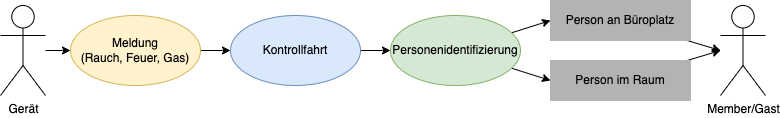
\includegraphics[width=15cm,height=15cm,keepaspectratio]{images/UC2_Diagramm_Notfall.png}
        \caption{Use Case 2 - Anwendungsfalldiagramm}
        \label{fig:uc2-emergency}
    \end{figure}
    \\
    %\linebreak
    Die Anwendungsfälle wurden so gewählt, da diese eine gewisse Komplexität mit sich bringen, die es mit der Steuerzentrale 
    abzudecken gilt.
    \\
    \linebreak
    Zur Stützung der textuellen Schilderung des zweiten Anwendungsfalls werden nachfolgend Diagramme dargestellt, die das Szenarien 
    widerspiegeln. Im Rahmen des \acs{RE} wurden hierfür ebenso eine konkrete Aufgabenbeschreibung, sowie eine User Story definiert. Diese sind dem 
    Anhang (siehe Anhang \ref{appendix:user-story-uc2}) zu entnehmen. Die folgenden Abbildungen stellen sich aus einem 
    Aktivitätsdiagramm, einem Sequenzdiagramm und einem Ablaufdiagramm zusammen: 
    %\\
    %Aus dem Kontext beider Anwendungsfälle, der vorangestellten Zielgruppenanalyse und den Experteninterviews werden in Abschnitt 
    %(\ref{sec:requirementsFinal}) die daraus identifizierten Anforderungen für die Steuerzentrale aufgeführt.
    